\section{Homework for chapter 1 (Introduction)}
\noindent \textbf{1.1 What are the differences between the brain of our human beings and electric brain (present computer)?}

\noindent Difference \# 1: Brains are analogue; computers are digital\\
Difference \# 2: The brain uses content-addressable memory\\
Difference \# 3: The brain is a massively parallel machine; computers are modular and serial.\\
Difference \# 4: Processing speed is not fixed in the brain; there is no system clock\\
Difference \# 5 – Short-term memory is not like RAM\\
Difference \# 6: No hardware/software distinction can be made with respect to the brain or mind.\\
Difference \# 7: Synapses are far more complex than electrical logic gates.\\
Difference \# 8: Unlike computers, processing and memory are performed by the same components in the brain.\\
Difference \# 9: The brain is a self-organizing system.\\
Difference \# 10: Brains have bodies.\\
Difference \# 11: The brain is much, much bigger than any [current] computer.\\
Difference \# 12:Computers rely on electricity, whereas humans rely on food\\
Difference \# 13: Computers have the potential to increase the speed of their impulse transmission exponentially as opposed to humans.\\
Difference \# 14: Computers have a better ability for multitasking.\\
Difference \# 15: Computers are good at computations and logic, while humans are exemplary in reasoning and imagination.

\noindent\textbf{1.2 What are tasks that the present computers perform well but our human beings perform
difficultly? And what are the tasks that our human beings perform very easily, while the
present computer performs very difficultly?}

\noindent Compared with the human brain, computers have the greatest advantage of performing high-frequency operations. The biggest drawback is that it is difficult for computers to make independent choices. Self-selection and effective learning are great advantages of the human brain.
\newpage
\noindent\textbf{1.3 What are the differences between the present computer and the present electronic dictionary?}

\noindent Computers and electronic dictionaries are different things. An electronic dictionary is a fixed-use electronic device that can only perform related operations of a dictionary and cannot be extended. Computers are different. Modern computers can be said to be a new software environment for working, learning, and running. On this basis, reasonable functions can be developed freely through software.

\noindent\textbf{1.4 Learning is one of the most significant ability of an artificial neural network. Supervised
learning and unsupervised learning are the two typical learning types of learning. Please try
your best to state supervised learning and unsupervised learning in precision respectively.}

\noindent The majority of practical machine learning uses supervised learning.Supervised learning is where you have input variables (x) and an output variable (Y) and you use an algorithm to learn the mapping function from the input to the output.The goal is to approximate the mapping function so well that when you have new input data (x) that you can predict the output variables (Y) for that data.It is called supervised learning because the process of an algorithm learning from the training data set can be thought of as a teacher supervising the learning process. We know the correct answers, the algorithm iteratively makes predictions on the training data and is corrected by the teacher. Learning stops when the algorithm achieves an acceptable level of performance.

\noindent Unsupervised learning is where you only have input data (X) and no corresponding output variables.The goal for unsupervised learning is to model the underlying structure or distribution in the data in order to learn more about the data.These are called unsupervised learning because unlike supervised learning above there is no correct answers and there is no teacher. Algorithms are left to their own devises to discover and present the interesting structure in the data.
\newpage
\noindent\textbf{1.5 Learning is one of the most significant ability of an artificial neural network. Hence the
questions are learning from where? Learning what? And learning to get what?}

\noindent In fact, the artificial neural network is a computer operation model that simulates the operation of the human brain. Through the learning ability of the perceptron, one such model is constructed. Then the perceptron is a simple linear binary classification model. It learns a parameter that minimizes the empirical risk by learning a large number of feature inputs and their labels. After learning, it acts on the new features to classify.

\noindent\textbf{1.6 Classification and regression are the two typical tasks that artificial neural networks can fulfill. Please define the two problems in perceptron respectively.}

\noindent It is often common to use neural network perceptrons to classify problems. In fact, all models that can be used for classification can basically be used for regression, so neural networks are no exception. The perceptron is a linear binary classification model driven by an error classification point. The classification result is obtained by adding the input weight to the activation function. Then, as long as the corresponding changes are made in the output layer of the neural network, a neural network for regression can be obtained.

\noindent \textbf{1.7 State a classification problem in perceptron which is a linearly separable problem.}

\noindent Since the perceptron is a classification model driven by misclassification points, the optimization algorithm uses stochastic gradient descent to iterate so that the training set samples have no misclassification points. If for a linear separable problem, we can prove that the algorithm is convergent. But for a linearly inseparable training sample set, the final algorithm must be oscillating, that is, it does not converge. So the original perceptron algorithm is a linear binary model.

\noindent\textbf{1.8 List as many as possible the application areas of the artificial neural networks.}

\noindent The application of neural networks is very extensive, and almost all classification problems can be used to do it. In recent years, neural networks have been widely used in computer vision, natural language processing, speech recognition, medical medicine, intelligent gaming, finance, and so on.


\newpage
\section{Homework for chapter 2 (tutorial)}
\noindent\textbf{1.1 Given two vectors X and Y, please give as many as possible ways for measuring the distance and/or similarity between X and Y.}

\noindent We can use the Lp distance (Minkowski Distance) to measure the distance between two vectors.
And if p=1  Manhattan Distance,p=2  Euclidean Distance ,p= Chebyshev Distance.
And the other ways to measuring are Standardized Euclidean distance,Mahalanobis Distance,
Hamming distance, and cosine similarity.

\noindent\textbf{1.2 Formulate the probability density function (pdf) of a uniformly distributed random variable ranged in [0,1], and derive from it the cdf(cumulative distribution function); formulate the pdf of a uniformly distributed random variable ranged in [5,10], and derive from it the cdf.}
\begin{align}
&x\sim U(0,1)&x\sim U(5,10)\nonumber\\
&PDF&PDF\nonumber\\
&f(x)= \begin{cases}
1& 0 \leq x \leq 1\\
0& others.
\end{cases}
&f(x)= \begin{cases}
\frac{1}{5}& 5 \leq x \leq 10\\
0& others.
\end{cases}\nonumber\\
&CDF&CDF\nonumber\\
&F(x)= \begin{cases}
0& x <0\\
x& 0 \leq x \leq 1\\
1& x >1
\end{cases}
&F(x)= \begin{cases}
0& x <5\\
\frac{x-5}{5}& 5 \leq x \leq 10\\
1& x >10
\end{cases}\nonumber
\end{align}

\noindent \textbf{1.3 Formulate the pdf f(x) of a Gaussian distributed random variable x with the means of 5 and standard deviation of 10. Calculate the derivative of the pdf with respect to the variable x.}

\begin{align}
&x\sim G(5,10^2)\nonumber\\
&f(x)= \frac{1}{\sqrt{2\pi}10}exp\Big(-\frac{(x-5)^2}{200}\Big) \nonumber \\
&f'(x)=\frac{1}{\sqrt{2\pi}10}exp\Big(-\frac{(x-5)^2}{200}\Big)\cdot -\frac{(x-5)}{100}\nonumber\\
&~~~~~~~~~=-\frac{(x-5)}{\sqrt{2\pi}1000} exp\Big(-\frac{(x-5)^2}{200}\Big) \nonumber
\end{align}
\newpage
\noindent \textbf{1.4 Formulate the pdf f(X) of a Gaussian distributed n-dimensional random vector X with the means of mu and the covariance matrix of Cx.}
\begin{align}
&X\sim G(\mu,\Sigma)\nonumber\\
&f(X)=\frac{1}{(2\pi)^\frac{n}{2}|\Sigma|^\frac{1}{2}}exp\Big(-\frac{1}{2}(X-\mu)^T\Sigma^{-1}(X-\mu)\Big) \nonumber
\end{align}

\noindent \textbf{1.5 Calculate the eigenvalues and eigenvectors of a symmetric 2x2 matrix C, where C=[1 2;2 1].}
\begin{align}
&A=\begin{bmatrix}
     ~~1 & 2~~ \\
     ~~2 & 1~~
   \end{bmatrix}\nonumber\\
&A\alpha=\lambda\alpha\nonumber\\
&(\lambda E-A)\alpha=0 \nonumber\\
&\lambda_1=3 ~~~\alpha_1=  [1,1]^T \nonumber\\
&\lambda_2=-1 ~~~\alpha_2=  [1,-1]^T \nonumber
\end{align}

\noindent\textbf{1.6 In what condition we say that two random variables are statistically independent, and in what condition we say that two random variables are statistically uncorrelated?}

\noindent If two random continuous variables x and y are statistically independent,\\
$f(x,y)=f_x(x)f_y(y)$.\\
If two random continuous discrete variables x and y are statistically independent,\\
$P(AB)=P(A)P(B)$.\\
If two random variables X and Y are statistically uncorrelated,\\
$r(X,Y)=\frac{Cov(X,Y)}{\sqrt{Var(X)Var(Y)}}$




\newpage
\section{Homework for chapter 3 (perceptron)}
%\noindent \textbf{Homework for chapter 3 (perceptron)~~~~~~~~~~~~~~~~~~~~~~~~~~~~~~~~~~\textbf{\textcolor{red}{冯哲 18031211394}}\\
\noindent \textbf{Paper sheet homework\\
3.1~(Duda’s~book,~p.316~1.) Consider~a~linear~machine~with~discriminant~functions~$~g_i(x)=W_ix_i,i=
1,...,c.~$Show that the decision regions are convex by showing that if $~W_1 \in \mathcal{R}~$ and
$~W_2 \in \mathcal{R}~$ then $~\lambda W_1 + (1 - \lambda)x_2 \in  \mathcal{R} ~,~0 \leq \lambda \leq 1~$.}
\begin{align}
&\because~ W_1,W_2 \in \mathcal{R} \nonumber\\
&\therefore~ y_i(W_1x_i)\geq 0~~~,~~~y_i(W_2x_i)\geq 0 \nonumber\\
&\because~ \exists \lambda \in [0,1]~,~(1-\lambda)\in [0,1] \nonumber\\
&\therefore~ \lambda y_i(W_1x_i) \geq 0~~,~~(1-\lambda) y_i(W_2x_i) \geq 0 \nonumber\\
&\therefore~ \lambda y_i(W_1x_i)+(1-\lambda) y_i(W_2x_i) \geq 0 \nonumber\\
&\therefore~ y_i(\lambda W_1+(1-\lambda)W_2)x_i\geq 0~,~~~i = 1,2,3,...,c \nonumber \\
&\therefore~ \lambda W_1+(1-\lambda)W_2 \in \mathcal{R} \nonumber
\end{align}
\textbf{3.2 ( Duda’s book, p317, 10.) Let the d components of x be either 0 or 1. Suppose we assign x to
$c_1$ if the number of non-zero components of x is odd, and to
$c_2$ otherwise. (This is called the d-bit parity
problem.) Show that this dichotomy is not linearly separable if $d > 1$.\\}

\noindent Our goal is to show that $\omega_1$ and $\omega_2$ are not linearly separable if $d > 1$. We prove
this by contradiction. Suppose that there exists a linear discriminant function$$g(x)=w^Tx+w_0$$
such that$$g(x)\geq 0~~for~~x\in \omega_1 $$$$g(x)< 0~~for~~x\in \omega_2$$
\textcircled{\footnotesize{1}}~b=0~~~,~~~$x=\{0,0,0,0,...,0,0,0\}$~~~$$g(0) = w^T 0 + w_0 = w_0 < 0$$
\textcircled{\footnotesize{2}}~b=1~~~,~~~$x=\{0,0,1,0,...,0,0,0\}$~~~$$g(x) = w_i + w_0 > 0$$
\textcircled{\footnotesize{3}}~b=2~~~,~~~$x=\{0,0,1,0,...,1,0,0\}$~~~$$g(x) = w_i + w_i +  w_0 < 0~,~for ~i \neq j$$
We summarize our results up to here as three equations:
$$ w_0 < 0$$
$$ w_i + w_0 > 0$$
$$ w_i + w_i +  w_0 < 0$$
for $i \neq j$. The first two of these imply
$$\underbrace{(w_i + w_0)} + \underbrace{(w_j + w_0)} + \underbrace{(-w_0)} > 0$$
$$>0~~~~~~~~~~~~~>0~~~~~~~~~~~~>0$$
$$ w_i + w_i +  w_0 < 0$$
 Thus our premise is false, and we have
proven that $\omega_1 ,\omega_2$ are not linearly separable if $d>1$.

\noindent\textbf{3.3 (Duke, p320, 25.) Consider the following six data points:\\
C1: (1, 2), (2, -4), (-3, -1)\\
C2: (2, 4), (-1, -5), (5, 0)\\
Are they linearly separable? If yes, try to learn a perceptron for discrimination of the two classes.}

\noindent By inspecting the plot of the points, we see that $\omega_1$ and $\omega_2$ are not linearly
separable, that is, there is no line that can separate all the $\omega_2$ points from all
the $\omega_2$ points..\\
 $$C1: x_1(0, -1), x_2(0, 0), x_3(-1, -1)~~~~~~~~~~1$$
 $$C2: x_4(~1, ~2), x_5(~2, ~~1), x_6(~~2, ~~2)~~~~~~-1$$
\indent,they are Linearly separable.
$$\eta = 1$$$$w := w + y_ix_i $$$$b := b + y_i$$
$$
\begin{tabular}{ccccc}
\hline k     &0&1      &2        &3        \\
\hline ~     & &$x_1$  &$x_5$    &$x_2$    \\
\hline $w_1$ &0&0      &-2       &-2       \\
\hline $w_2$ &0&-1     &-2       &-2       \\
\hline b     &0&1      &0        &1        \\
\hline
\end{tabular}
$$
separating line:$$x_2=-x_1+\frac{1}{2}$$

\noindent\textbf{3.4 State the following two generally used schemes for using multiple binary classifiers to solve a
multicategory problem: one-against-rest and one-against-one.}

\noindent The basic idea of binary classifier is to divide the data set into several binary classified data sets and apply binary classifier in combination. Typical methods include one-against-one and one-against-rest.

\noindent\textbf{ one against rest }method is to train a binary classifier for each class and binary classify it with all the other data. If there are K $(K > 2)$ classes, K classifiers need to be trained.

\noindent \textbf{one-against-one }method is to train a binary classifier between any two classes. If there are K classes, two classifiers of $\frac{K(K-1)}{2}$ need to be trained.


\newpage
\noindent\textbf{computer Homework}\\
3.5. \textbf{the data is in the following table:}
\begin{figure}[h]
  \includegraphics[width=0.6\textwidth]{3_5.eps}
%  \caption{}\label{}
\end{figure}
\textbf{Write a program to implement the Perceptron algorithm.\\
(a) Starting with a = 0, apply our program to the training data from $\omega_1$ and $\omega_2$ . Note the number of
iterations required for convergence.\\
(b) Apply our program to $\omega_3$ and $\omega_2$ . Again, note the number of iterations required for convergence.\\
(c) Explain the difference between the iterations required in the two cases.
}
\\


\noindent (a)(b) code:
\begin{lstlisting}
def trainPerceptron(dataMat, labelMat, eta):
    m, n = np.shape(np.mat(dataMat))
    weight = np.zeros(n)
    bias = 0
    flag = True
    t = 0
    while flag:
        for i in range(m):
            if np.any(labelMat[i] * (np.dot(weight, dataMat[i]) + bias) <= 0):
                weight = weight + eta * np.dot(labelMat[i],dataMat[i])
                bias = bias + eta * labelMat[i]
                print("weight, bias: ", end="\t")
                print(weight, end="\t")
                print(bias,end="\t")
                t =t+1
                print("#iteration: ",t,)
                flag = True
                break
            else:
                flag = False

    return weight, bias

if __name__ == "__main__":
    dataMat, labelMat = loadDataSet('w1_w2.txt')
    weight, bias = trainPerceptron(dataMat, labelMat, 1)

    dataMat, labelMat = loadDataSet('w2_w3.txt')
    weight, bias = trainPerceptron(dataMat, labelMat, 1)
\end{lstlisting}

\noindent \textcolor{red}{result:}\\\textbf{data set$\omega_1,\omega_2$}
\begin{lstlisting}
weight, bias:   [ 0.1  1.1]     1.0     #iteration:  1
weight, bias:   [-3.4 -3. ]     2.0     #iteration:  2
weight, bias:   [-3.3 -1.9]     3.0     #iteration:  3
weight, bias:   [ 3.5  5.2]     4.0     #iteration:  4
weight, bias:   [ 0.   1.1]     5.0     #iteration:  5
weight, bias:   [-7.1 -3.1]     4.0     #iteration:  6
weight, bias:   [-7. -2.]       5.0     #iteration:  7
weight, bias:   [-0.2  5.1]     6.0     #iteration:  8
weight, bias:   [-3.7  1. ]     7.0     #iteration:  9
weight, bias:   [ 3.1  8.1]     8.0     #iteration:  10
weight, bias:   [-0.4  4. ]     9.0     #iteration:  11
weight, bias:   [-3.9 -0.1]     10.0    #iteration:  12
weight, bias:   [ 2.9  7. ]     11.0    #iteration:  13
weight, bias:   [-0.6  2.9]     12.0    #iteration:  14
weight, bias:   [-7.7 -1.3]     11.0    #iteration:  15
weight, bias:   [-0.9  5.8]     12.0    #iteration:  16
weight, bias:   [-4.4  1.7]     13.0    #iteration:  17
weight, bias:   [ 2.4  8.8]     14.0    #iteration:  18
weight, bias:   [-1.1  4.7]     15.0    #iteration:  19
weight, bias:   [-4.6  0.6]     16.0    #iteration:  20
weight, bias:   [ 2.2  7.7]     17.0    #iteration:  21
weight, bias:   [-1.3  3.6]     18.0    #iteration:  22
weight, bias:   [-8.4 -0.6]     17.0    #iteration:  23
weight, bias:   [-1.6  6.5]     18.0    #iteration:  24
weight, bias:   [-5.1  2.4]     19.0    #iteration:  25
weight, bias:   [-3.7  6.7]     18.0    #iteration:  26
weight, bias:   [-10.8   2.5]   17.0    #iteration:  27
weight, bias:   [-4.   9.6]     18.0    #iteration:  28
weight, bias:   [-7.5  5.5]     19.0    #iteration:  29
weight, bias:   [-6.1  9.8]     18.0    #iteration:  30
weight, bias:   [-9.6  5.7]     19.0    #iteration:  31
weight, bias:   [ -2.8  12.8]   20.0    #iteration:  32
weight, bias:   [-6.3  8.7]     21.0    #iteration:  33
weight, bias:   [-13.4   4.5]   20.0    #iteration:  34
weight, bias:   [ -6.6  11.6]   21.0    #iteration:  35
weight, bias:   [-10.1   7.5]   22.0    #iteration:  36
weight, bias:   [ -8.7  11.8]   21.0    #iteration:  37
weight, bias:   [-15.8   7.6]   20.0    #iteration:  38
weight, bias:   [ -9.   14.7]   21.0    #iteration:  39
weight, bias:   [-12.5  10.6]   22.0    #iteration:  40
\end{lstlisting}
\begin{figure}[h]
  \centering
  \includegraphics[width=0.75\textwidth]{w1_w2.eps}
%  \caption{数据集$\omega_1,\omega_2$线性可分}
\end{figure}


\noindent \textbf{data set$\omega_2,\omega_3$}
\begin{lstlisting}
weight, bias:   [-7.1 -4.2]     -1.0    #iteration:  1
weight, bias:   [-5.7  0.1]     -2.0    #iteration:  2
weight, bias:   [-4.3  4.4]     -3.0    #iteration:  3
weight, bias:   [-7.3  1.5]     -2.0    #iteration:  4
weight, bias:   [-5.9  5.8]     -3.0    #iteration:  5
weight, bias:   [-8.9  2.9]     -2.0    #iteration:  6
weight, bias:   [-6.  5.]       -1.0    #iteration:  7
weight, bias:   [-3.1  7.1]     0.0     #iteration:  8
weight, bias:   [-10.2   2.9]   -1.0    #iteration:  9
weight, bias:   [-8.8  7.2]     -2.0    #iteration:  10
weight, bias:   [-5.9  9.3]     -1.0    #iteration:  11
weight, bias:   [-8.9  6.4]     0.0     #iteration:  12
weight, bias:   [-6.   8.5]     1.0     #iteration:  13
weight, bias:   [-9.   5.6]     2.0     #iteration:  14
weight, bias:   [-6.1  7.7]     3.0     #iteration:  15
weight, bias:   [-9.1  4.8]     4.0     #iteration:  16
weight, bias:   [-6.2  6.9]     5.0     #iteration:  17
\end{lstlisting}
\begin{figure}[h]
  \centering
  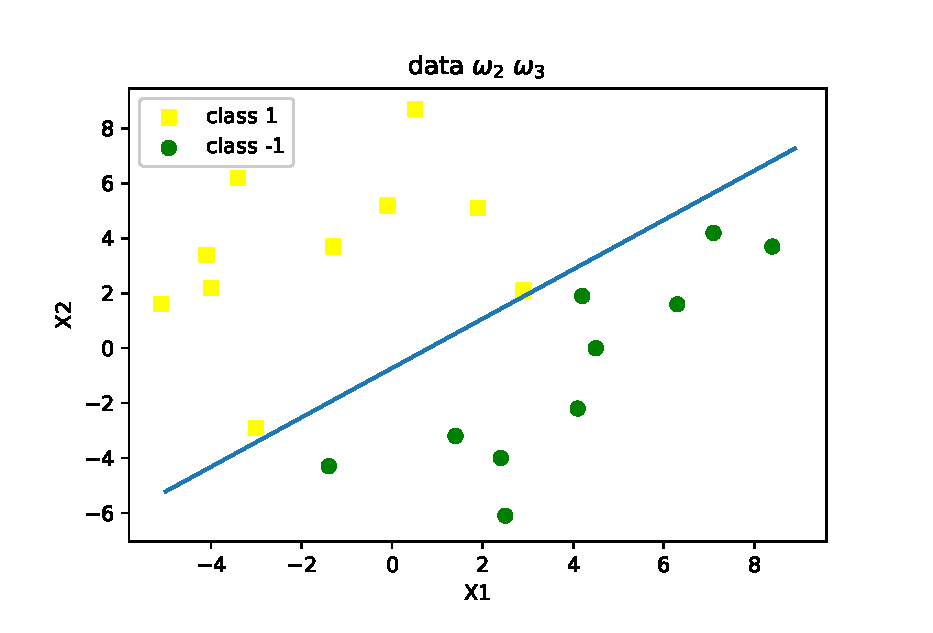
\includegraphics[width=0.75\textwidth]{w2_w3.eps}
%  \caption{数据集$\omega_2,\omega_3$线性可分}
\end{figure}

\noindent(c) The iterative solution process of the perceptron is only related to the error classification points. The iterative process under different data sets is definitely different, and the number of iterations is also related to the parameter $\eta$ setting. In fact, the final solution of the perceptron under the same data set also changes with the initial value of the parameter and the order of selection of the error classification point, that is,the solution of perceptron is not unique.


\newpage

\noindent \textbf{3.6 (Junying Zhang) A perceptron can be learnt to solve a linearly separable problem, and a generalized
perceptron can be learnt to solve a quadratic separable problem. Here is a two simple classification
problem: (a) two classes of samples in the training data are (1) scattered within two circulars centered in
(-10,0) and (10,0) both with the same variance of 1; (b) scattered within a circular centered in the origin
and within a half circular strip beside it.}

\begin{figure}[h]
  \centering
  \includegraphics[width=0.75\textwidth]{3_6.eps}
%  \caption{data distribution}
\end{figure}


\noindent\textbf{Derive Perceptron algorithm and Generalized Perceptron algorithm respectively and write two programs
to implement the algorithms for solving the above problems and exhibit your result on decision boundary
in figures.}

\noindent(a) For this problem, the two types of data sets are linearly separable, so the original algorithm using the perceptron can certainly converge.

\noindent code:
\begin{lstlisting}
def trainPerceptron(dataMat, labelMat, eta):
    m, n = np.shape(np.mat(dataMat))
    weight = np.zeros(n)
    bias = 0
    flag = True
    while flag:
        for i in range(m):
            if np.any(labelMat[i] * (np.dot(weight, dataMat[i]) + bias) <= 0):
                weight = weight + eta * np.dot(labelMat[i],dataMat[i])
                bias = bias + eta * labelMat[i]
                print("weight, bias: ", end="")
                print(weight, end="  ")
                print(bias)
                flag = True
                break
            else:
                flag = False

    return weight, bias
\end{lstlisting}

\noindent show result
\begin{figure}[!h]
  \centering
  \includegraphics[width=0.7\textwidth]{separated.eps}
%  \caption{}
\end{figure}

~\\

\noindent(b) For this problem, two sets of data  are linearly inseparable. Therefore, the original perceptron algorithm must not converge. We can use generalized linear discriminant function or duality algorithm with kernel function(RBF) of the perceptron, so I use the second method.

\noindent code :
\begin{lstlisting}
def kernelTrans(X, A, kTup): #calc the kernel or transform data to a higher dimensional space
    m,n = np.shape(X)
    K = np.mat(np.zeros((m,1)))
    if kTup[0]=='lin': K = X * A.T   #linear kernel
    elif kTup[0]=='rbf':
        for j in range(m):
            deltaRow = X[j,:] - A
#            print (K[j],deltaRow*deltaRow.T,j)
            K[j] = deltaRow*deltaRow.T
        K = np.exp(K/(-1*kTup[1]**2)) #divide in NumPy is element-wise not matrix like Matlab
    else: raise NameError('Houston We Have a Problem -- \
    That Kernel is not recognized')
    return K


def trainModel(dataMatIn,labelMatIn,eta,K):
    dataMat = np.mat(dataMatIn); labelMat = np.mat(labelMatIn).transpose()
    b = 0; m,n = np.shape(dataMat)
    alpha = np.mat(np.zeros((m,1)))
    flag = True
    while flag:
        for i in range(m):
            if  labelMatIn[i]*(float(np.multiply(alpha,labelMat).T*K[:,i]) + b)<= 0:
                alpha[i] = alpha[i] + eta
                b = b + eta * labelMat[i]
#                w = np.multiply(labelMat,alpha).T*dataMat
                print (i,alpha[i])
                flag = True
                break
            else:
                flag = False
#    w = (np.multiply(labelMat,alpha).T*dataMat).T
    return alpha
\end{lstlisting}

\noindent show result:
\begin{lstlisting}
0 [[ 1.]]
1 [[ 1.]]
15 [[ 1.]]
0 [[ 2.]]
54 [[ 1.]]
1 [[ 2.]]
20 [[ 1.]]
3 [[ 1.]]
13 [[ 1.]]
3 [[ 2.]]
13 [[ 2.]]
7 [[ 1.]]
403 [[ 1.]]
9 [[ 1.]]

alpha[alpha>0]
matrix([[ 2.,  2.,  2.,  1.,  1.,  2.,  1.,  1.,  1.,  1.]])
\end{lstlisting}

\begin{figure}[!h]
  \centering
  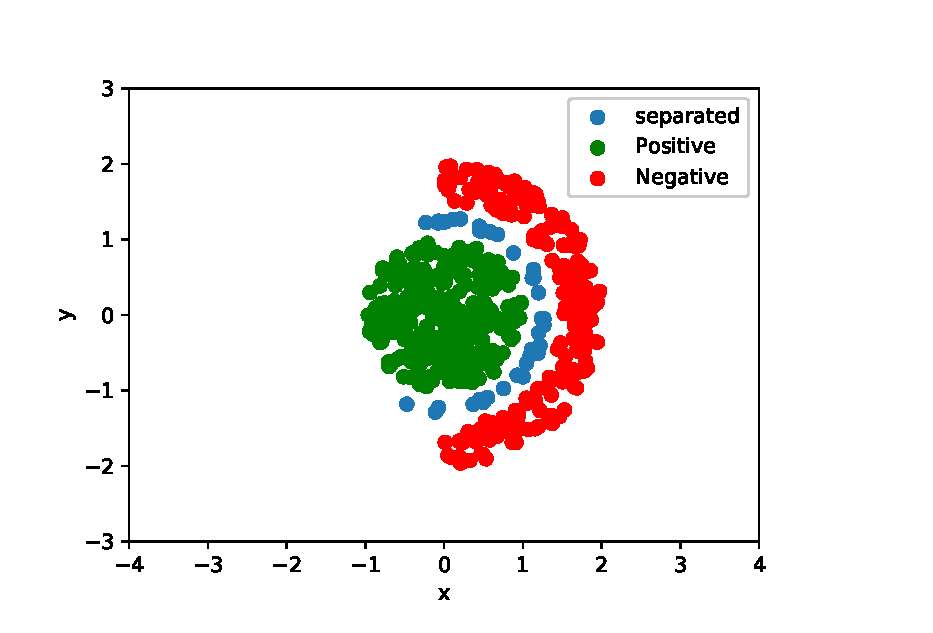
\includegraphics[width=0.7\textwidth]{Inseparated.eps}
%  \caption{}\label{}
\end{figure}


\newpage
\section{Homework for chapter 4 (MLP)}
\noindent \textbf{Paper sheet homework}\\
\noindent\textbf{4.1 Implementation of a 3D XOR problem. Here we have a three-dimensional XOR problem, in which the logic output y is an XOR operation on the three logic inputs x1,,xx23. The relation between the inputs and the output can be stated in the following table:
\begin{figure}[!h]
%  \centering
  \includegraphics[width=0.25\textwidth]{4_1.eps}
\end{figure}\\
Now the questions are\\
(1)	is it available to implement such an logic operation with a perceptron?}

The three-variable XOR problem is a nonlinear problem. The original perceptron is difficult to solve, it uses a nonlinear hypothesis to find a reasonable spatial display map, or introduces a kernel function space implicit mapping, or uses a multi-layer neural network.

\noindent\textbf{(2) is it available to implement such a logic operation with an MLP with only one hidden layer?}

A three-variable XOR problem can be solved with an MLP that contains only one hidden layer.

\noindent\textbf{(3) design an MLP with only one hidden layer to implement such a logic operation, including the structure of the MLP, and the parameters of the MLP.}

The essence of the first three variables XOR is the XOR of the two variables. The neural network constructed and parameters by XOR of two variables is as follows:\\
~\\
\centerline{
\begin{tabular}{cc|cc|cc}
\hline
Layer 1&~&Layer 1&~&Layer 2&~\\
\hline
$\theta^{(1)}_{10}$&-30&$\theta^{(1)}_{20}$&10&$\theta^{(2)}_{10}$&10\\
\hline
$\theta^{(1)}_{11}$&20&$\theta^{(1)}_{21}$&-20&$\theta^{(2)}_{11}$&-20\\
\hline
$\theta^{(1)}_{12}$&20&$\theta^{(1)}_{22}$&-20&$\theta^{(2)}_{12}$&-20\\
\hline
\end{tabular}}


\begin{figure}[!h]
  \centering
  \includegraphics[width=0.6\textwidth]{MLP.png}
\end{figure}

Decision-making process:
~\\

\centerline{
\begin{tabular}{cc|cc|c}
\hline
$x_1$&$x_2$&$a^{(1)}_1$&$a^{(1)}_2$&$h_\theta(x)$\\
\hline
0&0&0&1&0\\
\hline
0&1&0&0&1\\
\hline
1&0&0&0&1\\
\hline
1&1&1&0&0\\
\hline
\end{tabular}}
~\\
Finally, use each two XOR to solve the three-variable XOR problem.

\noindent\textbf{4.2 Show that if the activation function of the hidden units is linear, a 3-layer (1 input layer x, 1
hidden layer h and 1 output layer y) network is equivalent to a 2-layer one. Use your result to
explain why a three-layer network with linear hidden units cannot solve a non-linearly separable
problem such as XOR.}

The above two-layer network is actually a perceptron. Since the original perceptron can only solve the linear classification problem, and the XOR problem is a linear inseparable problem, the perceptron cannot solve the problem.

\noindent\textbf{4.3 Consider a standard three-layer backpropagation net with d input units, n hidden units, c output
H units. \\\noindent (a) How many weights are in the net? \\\noindent(b) draw the relation between the number of weights and the number of hidden neurons.}

(a) \#weights are $n_H*d+n_H*c$\\
\indent (b) $h(n_H) = (d+c)*n_H$  Linear relationship.


\noindent\textbf{4.4 Express the derivative of a sigmoid in terms of the sigmoid itself in the following two cases (for positive constants a and b): \\
(a)A sigmoid that is purely positive:$$f(x)=\frac{1}{1+\exp(ax)}$$\\
(b) An anti-symmetric sigmoid: $$f(x)=a\tanh(bx)$$}

(a)$$\frac{df(x)}{dx} = -a(\frac{1}{1+\exp(ax)})^2e^{ax}=-af(x)(1-f(x))$$

(b)$$\frac{df(x)}{dx} = -2b^2a\tanh(bx)(1-\tanh^2(bx))$$



\newpage
\noindent \textbf{4.5 Consider a general constant matrix K and variable vector parameters x.\\
(a) Write in summation notation with components explicit, and derive the formula
for the derivative:$$\frac{d}{dx}x^TKx = (K+K^T)x$$
(b) Show simply that for the case where K is symmetric (as for instance the Hessian
matrix $H = H^T$ ), we have:$$\frac{d}{dx}x^THx = 2Hx$$}
\begin{figure}[!h]
  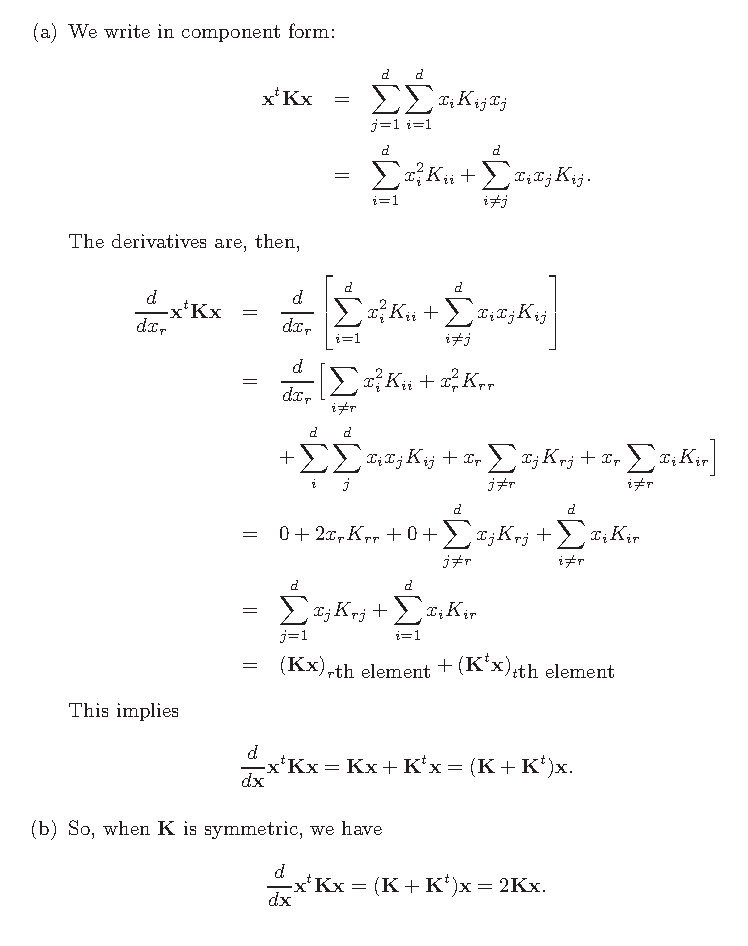
\includegraphics[width=0.8\textwidth]{37.eps}
\end{figure}

\newpage
\noindent \textbf{Computer homework}\\
\noindent \textbf{4.6 (Duda’s book, p.396, 4.)Write a backpropagation program for a 2-2-1 network with bias to solve the
XOR problem. Show the input-to-hidden weights and analyze the function of each hidden unit.}

\noindent Actually, this answer is same with problem 4.1. and 2-2-1 network as shown.
~\\
~\\

\begin{figure}[!h]
  \centering
  \includegraphics[width=0.6\textwidth]{MLP.png}
\end{figure}
~\\

\noindent main function:
\begin{lstlisting}
def fit(X, Y, w):
   # now each para has a grad equals to 0
    w_grad = ([np.mat(np.zeros(np.shape(w[i]))) for i in range(len(w))])  # len(w) equals the layer number
    m, n = X.shape
    h_total = np.zeros((m, 1))  #  m*1, probability
    for i in range(m):
        x = X[i]
        y = Y[0,i]
        # forward propagate
        a = x
        a_s = []
        for j in range(len(w)):
            a = np.mat(np.append(1, a)).T
            a_s.append(a)
            z = w[j] * a
            a = sigmoid(z)
        h_total[i, 0] = a
        # back propagate
        delta = a - y.T
        w_grad[-1] += delta * a_s[-1].T
        for j in reversed(range(1, len(w))):
            delta = np.multiply(w[j].T*delta, s_prime(a_s[j]))
            w_grad[j-1] += (delta[1:] * a_s[j-1].T)
    w_grad = [w_grad[i]/m for i in range(len(w))]
    J = (1.0 / m) * np.sum(-Y * np.log(h_total) - (np.array([[1]]) - Y) * np.log(1 - h_total))
    return {'w_grad': w_grad, 'J': J, 'h': h_total}

X = np.mat([[0,0],
            [0,1],
            [1,0],
            [1,1]])
Y = np.mat([0,1,1,0])
layers = [2,2,1]
epochs = 3000
alpha = 0.6
w = init_weights(layers, 1)
result = {'J': [], 'h': []}
w_s = {}
for i in range(epochs):
    fit_result = fit(X, Y, w)
    w_grad = fit_result.get('w_grad')
    J = fit_result.get('J')
    h_current = fit_result.get('h')
    result['J'].append(J)
    result['h'].append(h_current)
    for j in range(len(w)):
        w[j] -= alpha * w_grad[j]
    if i == 0 or i == (epochs - 1):
#        print('w_grad', w_grad)
        w_s['w_' + str(i)] = w_grad[:]

plt.plot(result.get('J'))
plt.show()
\end{lstlisting}

\newpage
\noindent When the learning rate is set too small and the number of iterations is not set enough, there will be no convergence,or local optimum. As shown:

\begin{figure}[!h]
\begin{minipage}
{0.5\linewidth}
\centering
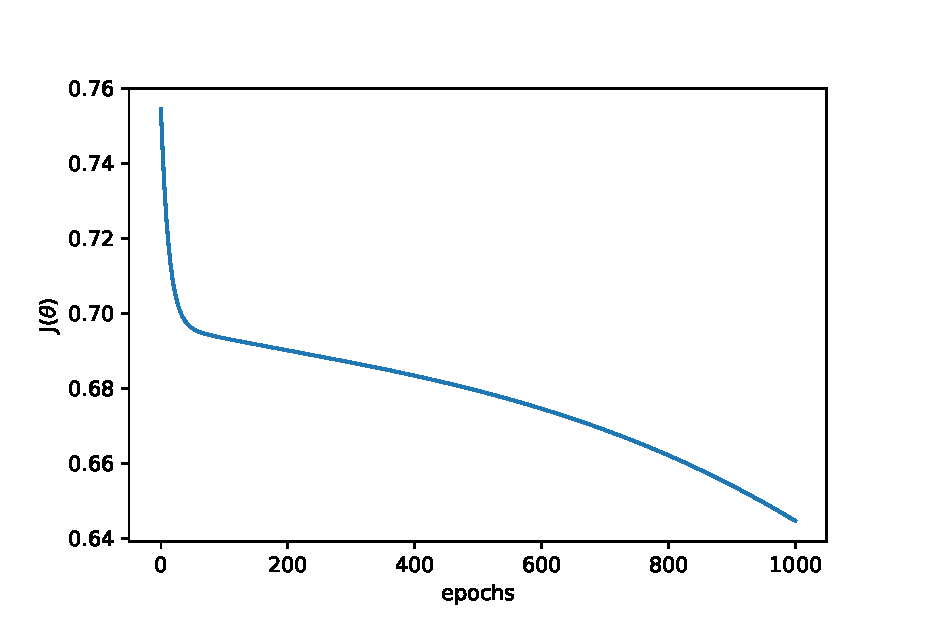
\includegraphics[width=3.1in]{NoConverge.eps}
\end{minipage}
%
\begin{minipage}
{0.5\linewidth}
\centering
\includegraphics[width=3.1in]{LocalOptimum.eps}
\end{minipage}
\end{figure}

\noindent By adjusting to a good number of iterations and learning rates, there will still be occasional traps in the local optimal solution. This is due to the fact that it is also closely related to the initial value. As shown

\begin{figure}[!h]
\begin{minipage}
{0.5\linewidth}
\centering
\includegraphics[width=3.1in]{SomeLocalOptimum.eps}
\end{minipage}
%
\begin{minipage}
{0.5\linewidth}
\centering
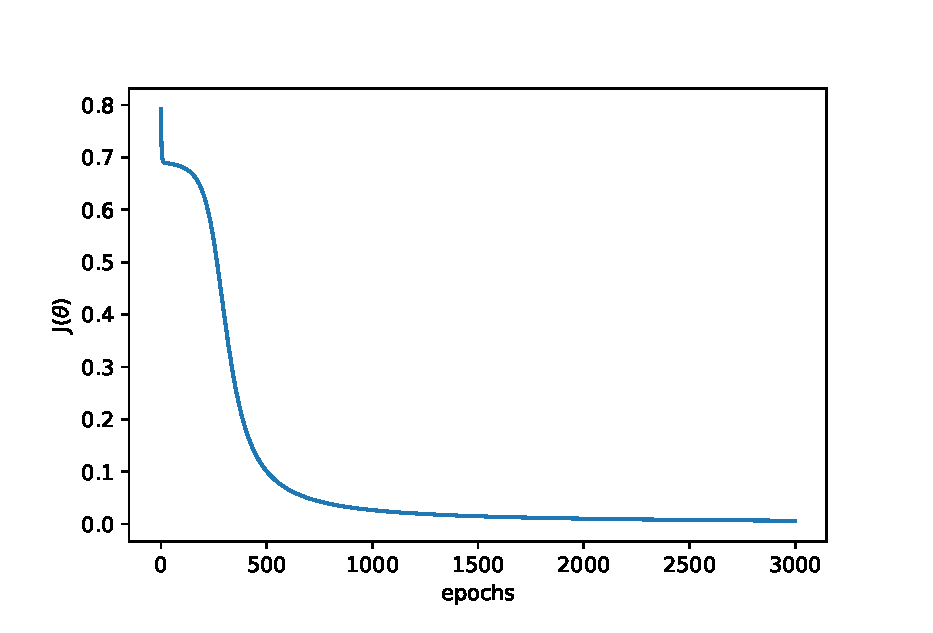
\includegraphics[width=3.1in]{result.eps}
\end{minipage}
\end{figure}

\noindent Finally, when the $\eta = 0.6$, and $epochs = 3000$ is displayed, the initialization value and final value of the weight parameter:
~\\

\begin{lstlisting}
{'w_0': [matrix([[-0.00160309,  0.00402848, -0.00035563],
                 [ 0.00051501, -0.00189287, -0.00094397]]),
         matrix([[ 0.0172645 ,  0.01289784,  0.01025378]])],

'w_2999': [matrix([[-0.00021253,  0.00045426, -0.00047387],
                   [-0.00031218, -0.00062748,  0.00062853]]),
           matrix([[-0.00220671,  0.00147604,  0.00145586]])]}
\end{lstlisting}
\newpage
Decision-making process:
~\\

\centerline{
\begin{tabular}{|cc|c|}
\hline
$x_1$&$x_2$&$h_\theta(x)$\\
\hline
0&0&0.01507\\
\hline
0&1&0.98856\\
\hline
1&0&0.98850\\
\hline
1&1&0.01642\\
\hline
\end{tabular}}
~\\


\noindent \textbf{4.7 Write a basic backpropagation program for a 3-3-1 network with bias to solve the
three-bit parityproblem, i.e., return a +1 if the number of input units that are high
is even, and -1 if odd.\\
(a) Show the input-to-hidden weights and analyze the function of each hidden unit.\\
(b) Retrain several times from a new random point until you get a local (but not
global) minimum. Analyze the function of the hidden units now.\\
(c) How manypatterns are properlyclassified for your local minimum?}

The core of solving the three-variable parity check problem using the 3-3-1 neural network is similar to the previous one, and the back propagation algorithm is used to minimize the loss function.

\noindent main process:
\begin{lstlisting}
X = np.mat([[0,0,0],
            [0,0,1],
            [0,1,0],
            [0,1,1],
            [1,0,0],
            [1,0,1],
            [1,1,0],
            [1,1,1],])
Y = np.mat([1,0,0,1,0,1,1,0])
layers = [3,3,1]
epochs = 3000
alpha = 0.6
w = init_weights(layers, 1)
result = {'J': [], 'h': []}
w_s = {}
for i in range(epochs):
    fit_result = fit(X, Y, w)
    w_grad = fit_result.get('w_grad')
    J = fit_result.get('J')
    h_current = fit_result.get('h')
    result['J'].append(J)
    result['h'].append(h_current)
    for j in range(len(w)):
        w[j] -= alpha * w_grad[j]
    if i == 0 or i == (epochs - 1):
#        print('w_grad', w_grad)
        w_s['w_' + str(i)] = w_grad[:]
\end{lstlisting}

\noindent Local optimum and optimal situation:
\begin{figure}[!h]
\begin{minipage}
{0.5\linewidth}
\centering
\includegraphics[width=3.1in]{LocalOptimum2.eps}
\end{minipage}
%
\begin{minipage}
{0.5\linewidth}
\centering
\includegraphics[width=3.1in]{result2.eps}
\end{minipage}
\end{figure}

\noindent Local optimum and optimal situation weights:
\begin{lstlisting}
#Local optimum
{'w_0': [matrix([[-0.00965728, -0.00498227, -0.00432775, -0.00532431],
                 [ 0.00390881,  0.00214983,  0.00220814,  0.00197096],
                 [-0.01433964, -0.00771318, -0.00822238, -0.00741432]]),
         matrix([[-0.09794386, -0.02150587, -0.04508723, -0.03333154]])],

'w_2999': [matrix([[ -2.31463002e-03,   2.73389956e-03,   2.19245855e-03,
          -3.05958861e-03],
                   [ -1.20327006e-04,   5.93500754e-04,   2.06230228e-04,
          -3.78728393e-04],
                   [  3.24364244e-05,  -1.81457519e-04,  -6.37281831e-04,
           1.23834517e-03]]),
           matrix([[ 0.00078726, -0.0018065 ,  0.00114248, -0.000721  ]])]}

#optimal situation
{'w_0': [matrix([[ 0.0031695 , -0.00222643,  0.00644728, -0.00209555],
                 [ 0.00379564, -0.00168618,  0.00699103, -0.00309226],
                 [-0.00527478, -0.00078626, -0.0059792 , -0.00107995]]),
         matrix([[-0.02576137, -0.02303488, -0.02278934, -0.00840099]])],

'w_2999': [matrix([[  1.25629498e-04,  -6.07297784e-04,  -5.31491848e-04,
           8.73974056e-04],
                   [  5.36966594e-05,   8.70982128e-04,  -4.24791065e-04,
          -5.49887584e-04],
                   [  3.64388345e-05,   2.73108890e-04,  -6.83896015e-04,
           3.20232681e-04]]),
           matrix([[-0.00099446,  0.0018958 ,  0.00184206, -0.00176173]])]}
\end{lstlisting}

\noindent optimal situation training data output:
\begin{lstlisting}
#First iteration
[[ 0.47389793]
 [ 0.51023924]
 [ 0.40658669]
 [ 0.42947268]
 [ 0.51651459]
 [ 0.55465096]
 [ 0.43271946]
 [ 0.46982745]]

#Last iteration
 [[ 0.99784547]
  [ 0.01401809]
  [ 0.01908374]
  [ 0.98290443]
  [ 0.01461569]
  [ 0.9772841 ]
  [ 0.98386423]
  [ 0.00242857]]
\end{lstlisting}






\newpage
\section{Homework for chapter 5 (KMeans)}
\noindent \textbf{5.1 Let $x_1,...,x_n$ be nd-dimensional samples and $\Sigma$ be any non-singular d-by-d matrix. Show that the vector x that minimizes
$$\sum_{k=1}^{m}(x_k-x)^t\Sigma^{-1}(x_k-x)$$
is  the sample mean,$\hat{x} = \frac{1}{n}\sum_{k=1}^{n}x_k$}

let the mean value be denoted$$\hat{x}=\sum_{i=1}^{m}x_k$$
\begin{align}
&\frac{1}{n}\sum_{k=1}^{n}(x_k-x)^T\Sigma^{-1}(x_k-x)\nonumber\\
&=\frac{1}{n}\sum_{k=1}^{n}(x_k-\hat{x}+\hat{x}-x)^T\Sigma^{-1}(x_k-\hat{x}+\hat{x}-x)\nonumber\\
&=\frac{1}{n}\sum_{k=1}^{n}(x_k-\hat{x})^T\Sigma^{-1}(x_k-\hat{x})\nonumber\\
&+2(\hat{x}-x)^T\Sigma^{-1}\sum_{k=1}^{n}(x_k-\hat{x})+n(\hat{x}-x)^T\Sigma^{-1}(\hat{x}-x)\nonumber\\
&=\frac{1}{n}\sum_{k=1}^{n}(x_k-\hat{x})^T\Sigma^{-1}(x_k-\hat{x})+(\hat{x}-x)^T\Sigma^{-1}(\hat{x}-x)\nonumber\\
&\geq \frac{1}{n}\sum_{k=1}^{n}(x_k-\hat{x})^T\Sigma^{-1}(x_k-\hat{x})\nonumber
\end{align}\\
where we used:
$$\sum_{i=1}^{m}(x_k-\hat{x})=0$$
Since $\Sigma$ is positive definite,we have:
$$(\hat{x}-x)^T\Sigma^{-1}(\hat{x}-x)\geq 0$$
So  $$\sum_{k=1}^{m}(x_k-x)^t\Sigma^{-1}(x_k-x)$$ is minimized at $x=\hat{x}$.


\newpage
\section{Homework for chapter 6 (RBF)}
\noindent \textbf{5.1 (Haykin’s book, p.334, 5.3) Consider an exact solution of the XOR problem using an RBF
network with four hidden units, with each radial basis function center being determined by each
piece of input data. The four possible input patterns are defined by (0,0), (0,1), (1,0), and (1,1),
which represent the cyclically ordered corners of a square.\\
(a) Construct the interpolation matrix $~\Phi~$ for the resulting RBF network. Hence, compute the
inverse matrix �$\Phi^{-1}$ .\\
(b) Calculate the linear weights of the output layer of the network.}

\noindent(a) We know that the radial basis function is$$\phi(x) = e^{-|x-c_i|^2}$$
$~c_1,c_2,c_3,c_4 = (0,0),(0,1),(1,0),(1,1)~$ \\
$$X = \begin{bmatrix}
      0 & 0 \\
      0 & 1 \\
      1 & 0 \\
      1 & 1
    \end{bmatrix}~~~~~~~~~~~~~~~~~
Y = \begin{bmatrix}
      0 \\
      1 \\
      1 \\
      0
    \end{bmatrix}$$\\
$$\Phi = \begin{bmatrix}
              1.          &0.36787944  &0.36787944  &0.13533528 \\
              0.36787944  &1.          &0.13533528  &0.36787944 \\
              0.36787944  &0.13533528  &1.          &0.36787944 \\
              0.13533528  &0.36787944  &1.36787944  &1.
            \end{bmatrix}$$
So $$\Phi^{-1} = \begin{bmatrix}
              1.33753306 &-0.49205091 &-0.49205091  &0.18101542 \\
              -0.49205091 & 1.33753306  &0.18101542 &-0.49205091 \\
              -0.49205091  &0.18101542 & 1.33753306 &-0.49205091 \\
              0.18101542 &-0.49205091 &-0.49205091  &1.33753306
            \end{bmatrix}$$

\noindent(b)  We know $$~\Phi W = Y ~$$ So $$W =\phi^{-1} Y$$
That is $$W = \begin{bmatrix}
           -0.98410183 \\
           1.51854847 \\
           1.51854847 \\
           -0.98410183
         \end{bmatrix}$$

\noindent \textbf{5.2 (Haykin’s book, p.335, 5.4) The Gaussian function is the only radial basis function which is
factorable. Using this property of the Gaussian function, show that the function G(x,t) defined
as a multivariate Gaussian distribution may be factorized as follows:
$$G(x,t) = \Pi_{i=1}^{m}G(x_i,t_i)$$
where $x_i$ and $t_i$ are the i th elements of the m -by-1 vector x and t.}


\noindent
\begin{align}
d(x,t)&= (x-t)^T\Sigma^{-1}(x-t)\nonumber \\
&=\begin{bmatrix}
    x_1-t_1 & x_2-t_2 & \cdots & x_m-t_m
  \end{bmatrix}\begin{bmatrix}
                                     \frac{1}{\sigma_1^2} & 0 & \cdots & 0 \\
                                     0& \frac{1}{\sigma_2^2} & \cdots & 0 \\
                                     \vdots & \vdots & \ddots & \vdots \\
                                     0 & 0 & \cdots & \frac{1}{\sigma_m^2}
                                   \end{bmatrix}\begin{bmatrix}
                                                  x_1-t_1 \\
                                                  x_2-t_2 \\
                                                  \vdots \\
                                                  x_m-t_m
                                                \end{bmatrix}\nonumber\\
&=(\frac{x_1-t_1}{\sigma_1^2})^2+(\frac{x_2-t_2}{\sigma_2^2})^2+\cdots+(\frac{x_m-t_m}{\sigma_m^2})^2\nonumber\\
G(x;t,\Sigma)&=\frac{1}{(2\pi)^{n/2}|\Sigma|^{1/2}}\exp\Big(-\frac{1}{2}(x-t)^T\Sigma^{-1}(x-t)\Big)\nonumber\\
&=\frac{1}{(2\pi)^{n/2}|\Sigma|^{1/2}}\exp\Big(-\frac{1}{2}d(x,t)^2\Big)\nonumber\\
&=\frac{1}{(2\pi)^{n/2}|\Sigma|^{1/2}}\exp\Big(-\frac{1}{2}\big[(\frac{x_1-t_1}{\sigma_1^2})^2+(\frac{x_2-t_2}{\sigma_2^2})^2+\cdots+(\frac{x_m-t_m}{\sigma_m^2})^2\big]\Big)\nonumber\\
&=\frac{1}{\sqrt{2\pi}\sigma_1}\exp\Big({-\frac{1}{2}(\frac{x_1-t_1}{\sigma_1})^2}\Big)\cdots\frac{1}{\sqrt{2\pi}\sigma_m}\exp\Big({-\frac{1}{2}(\frac{x_m-t_m}{\sigma_m})^2}\Big)\nonumber\\
&=\Pi_{i=1}^mG(x_i;t_i,\Sigma)\nonumber
\end{align}
So$$G(x;t,\Sigma)=\Pi_{i=1}^mG(x_i;t_i,\Sigma)$$



\newpage
\section{Homework for chapter 7 (SVM)}
\noindent\textbf{Paper sheet homework}\\
\noindent \textbf{6.1 (Haykin’s book, pp.357, 6.5) Now let us revisit Exclusive OR (XOR) problem. Let the kernel
function to be $K(x,x_i)=(1+xx_i)^2$, where $x=(x_1,x_2)^T$ and $x_i=(x_{1i},x_{2i})^T$. Please give the kernel
matrix for the four logic input samples for this problem, and write down the corresponding objective
function of the dual problem.}

\noindent we know the duality problem is
\begin{align}
\min\limits_{\alpha}~~ \frac{1}{2}\sum_{i=1}^{m}&\sum_{j=1}^{m}\alpha_i\alpha_jy_iy_jK(x_i,x_j)-\sum_{i=1}^{m}\alpha_i\nonumber\\
&s.t.~~~~~~\sum_{i=1}^{m}\alpha_iy_i = 0\nonumber\\
&0\leq\alpha_i\leq C,~~~i=1,2,\cdots,m \nonumber
\end{align}
and training samples and corresponding labels
$$X = \begin{bmatrix}
      0 & 0 \\
      0 & 1 \\
      1 & 0 \\
      1 & 1
    \end{bmatrix}~~~~~~~~~~~~~~~~~
Y = \begin{bmatrix}
      0 \\
      1 \\
      1 \\
      0
    \end{bmatrix}$$\\
First, the kernel function is $K(x,x_i)=(1+xx_i)^2$ and the kernel matrix is easy to get.
$$K =\begin{bmatrix}
       1 & 1 & 1 & 1 \\
       1 & 4 & 1 & 4 \\
       1 & 1 & 4 & 4 \\
       1 & 4 & 4 & 9
     \end{bmatrix}$$\\
Bring the sample and kernel matrix into the super dual problem.
\begin{align}
~~~~~~~~~\min\limits_{\alpha}~~ &2\alpha_2^2+2\alpha_3^2+\alpha_2\alpha_3-\sum_{i=1}^{4}\alpha_i\nonumber\\
&s.t.~~~~~~\alpha_2+\alpha_3 = 0\nonumber\\
&0\leq\alpha_i\leq C,~~~i=1,2,3,4 \nonumber
\end{align}

\newpage
\noindent\textbf{6.2 (Haykin’s book, pp.348, 6.6) The inner-product kernel $K(x_i,x_j)$ is evaluated over a training sample
set of size N , yielding the N -by- N matrix
$$K = \{K_{ij}\}^N_{(i,j)=1}$$
where $K_{ij}=K(x_i,x_j)$. The matrix K is positive in that all of its elements have positive values. Using
the similarity transformation
$$K = Q\Lambda Q^T$$
where $\Lambda$ is a diagonal matrix of eigenvalues and Q is a matrix made up of the corresponding
eigenvectors, formulate an expression for the inner-product kernel $K(x_i,x_j)$ in terms of the eigenvalues
and eigenvectors of the matrix K . What conclusions can you draw from this representation?}

\noindent The conclusion that can actually be obtained is the Mercer theorem:\\
If the function K is a mapping on $\mathbb{R}^n \times \mathbb{R}^n \rightarrow \mathbb{R}$ (that is, mapping from two n-dimensional vectors to a real number field). Then if K is a valid kernel function (also known as the Mercer kernel function), then if and only for the training example $\{x^{(1)},x^{(2)},\cdots,x^{(m)}\}$, its corresponding kernel function matrix is symmetric semi-definite.\\
prove Mercer theorem:
\begin{align}
\Lambda&=Z^TKZ\nonumber\\
&=\sum_i\sum_jz_iK_{ij}z_j\nonumber\\
&=\sum_i\sum_jz_i\phi(x^{(i)})^T\phi(x^{(j)})z_j\nonumber\\
&=\sum_i\sum_jz_i\sum_k\phi_k(x^{(i)})\phi_k(x^{(j)})z_j\nonumber\\
&=\sum_k\sum_i\sum_jz_i\phi_k(x^{(i)})\phi_k(x^{(j)})z_j\nonumber\\
&=\sum_k\Big(\sum_iz_i\phi_k(x^{(i)})\Big)^2\nonumber\\
&\geq 0 \nonumber
\end{align}
Therefore, $\Lambda$ is semi-definite, so K is also semi-definite.

\noindent \textbf{6.3 (Haykin’s book, pp.348, 6.7) \\(a) prove the unitary invariance property of the inner-product kernel
$K(x,x_i)$; that is,
$$K(x,x_i)=K(Qx,Qx_i)$$
where Q is a unitary matrix defined by $Q^{-1}=Q^T$.\\
(b) Demonstrate that the RBF kernel satisfies this property.}

\noindent(a) The kernel function has two important properties: translation invariance and rotation invariance.This problem is rotation invariance.because of $Q^{-1}=Q^T$,Q is the rotation matrix.
$$<x,x_1> = <Qx,Qx_1>$$
The implicit feature mapping of kernel functions is a rotation of low-dimensional rotation to high-dimensional space.
$$K(x,x_i)=K(Qx,Qx_i)$$

\noindent(b)Gaussian kernel function $$K(x,z)=\exp\Big(-\frac{||x-z||^2}{2\sigma^2}\Big)$$
$$K(Qx,Qx_1)=\exp\Big(-\frac{||Qx-Qx_1||^2}{2\sigma^2}\Big)~~~~~~~~~~~~~~~~~~~~~~~~~~~~~~~~~~~~~~~~~~~~~~~~~~~~~~~~~~~~~~~~~~$$
$$=\exp\Big(-\frac{||Q||^2||x-x_1||^2}{2\sigma^2}\Big)=\exp\Big(-\frac{||x-x_1||^2}{2\sigma^2}\Big)$$
$$=K(x,x_1)~~~~~~~~~~~~~~~~~~~~~~~~~~~~~~~~~~~~~~~~~~~~~~~~~~~~~~~~~~~~~~~~~~~~~~$$
where we used $$||Q|| = 1,~~~~~Q^{-1} = Q^T$$

\noindent \textbf{6.4 Throughout the chapter we discussed the use of a support vector machine for binary classification.
Discuss how a support vector machine can be used to solve an M -ary pattern classification problem,
where M $>$� 2.}

\noindent Multi-classification of support vector machines is implemented indirectly. There are two ways, one-V-one and one-V-rest.\\
one-V-one:~~~
For the k-type data set, the SVM is designed separately for each of the two types of samples for classification. In the end, k(k-1)/2 classifiers must be designed and finally selected by voting.\\
one-V-rest:~~~
Classify a class as a positive class, and the rest are negative. Finally, a Huffman decision tree is generated.

\newpage
\noindent \textbf{Computer exercises\\
6.5 (Hykin’s book, pp.349, 6.9) The inner-product kernel for a polynomial learning machine used to
solve the XOR problem is defined by
$$K(x,x_i)=(1+x^Tx_i)^P$$
What is the minimum value of power p for which the XOR problem is solved? Assume that p is a
positive integer. What is the result of using a value for p larger than the minimum?}

\noindent main process:
\begin{lstlisting}
from sklearn.svm import SVC
import numpy as np

X = np.array([[0,0], [0,1], [1,0], [1,1]])
y = np.array([0, 1, 1, 0])

for j in range(100):
    clf = SVC(C=1000000,kernel='poly',degree=j)
    clf.fit(X, y)
    trainingAccuracy = 0
    trainingAccuracy += sum(y == clf.predict(X))/len(X)
    print ('power = ',j,'\taccuracy = ',trainingAccuracy)
\end{lstlisting}

\noindent result
\begin{lstlisting}
power =  0      accuracy =  0.5
power =  1      accuracy =  0.5
power =  2      accuracy =  1.0
power =  3      accuracy =  1.0
power =  4      accuracy =  1.0
power =  5      accuracy =  1.0
power =  6      accuracy =  1.0
power =  7      accuracy =  1.0
power =  8      accuracy =  1.0
power =  9      accuracy =  1.0
power =  10     accuracy =  1.0
power =  11     accuracy =  1.0
power =  12     accuracy =  1.0
power =  13     accuracy =  1.0
power =  14     accuracy =  1.0
\end{lstlisting}
\newpage
\begin{lstlisting}
power =  15     accuracy =  1.0
power =  16     accuracy =  1.0
power =  17     accuracy =  1.0
power =  18     accuracy =  1.0
power =  19     accuracy =  0.75
power =  20     accuracy =  0.75
power =  21     accuracy =  0.75
power =  22     accuracy =  0.75
power =  23     accuracy =  0.75
power =  24     accuracy =  0.75
power =  25     accuracy =  0.75
power =  26     accuracy =  0.75
power =  27     accuracy =  0.75
power =  28     accuracy =  0.75
power =  29     accuracy =  0.75
power =  30     accuracy =  0.75
power =  31     accuracy =  0.75
power =  32     accuracy =  0.75
power =  33     accuracy =  0.75
power =  34     accuracy =  0.75
power =  35     accuracy =  0.75
power =  36     accuracy =  0.75
power =  37     accuracy =  0.75
power =  38     accuracy =  0.75
power =  39     accuracy =  0.75
power =  40     accuracy =  0.75
\end{lstlisting}
we set C = 1000000,~~transform soft margin SVM to the hard margin SVM.This means that the classifier is focused on classifying the training set samples correctly.

\noindent From the program results, the exponential minimum of the polynomial kernel function to solve the XOR problem is 2.

\noindent From the results, when $1<power<19$, The classifier can solve the XOR problem. In fact this is related to the setting of the C value. I think that when setting C to infinity, when $1<power$,it can solve the XOR problem.


\newpage
\section{Homework for chapter 8 (SOM)}
\noindent\textbf{Paper sheet homework\\
9.1 (Haykin’s book, pp.479, 9.3) It is sometimes said that the SOM algorithm preserves the topological
relationships that exist in the input space. Strictly speaking, this property can be guaranteed only for an
input space of equal or lower dimensionality than that of the neural lattice. Discuss the validity of this
statement}

\noindent Consider the "Peano curve" shown in Figure 1c. The self-organizing map has a one-dimensional
lattice that is taught with two-dimensional data. We can see that the data points inside the circle
map to either unit A or unit B on the map. Some of the data points are mapped very far from
each other on the lattice of the SOM even though they are close by in the input space. Thus the
topological relationships are not preserved by the SOM. This is true in general for any method that
reduces dimensionality. It is not possible to preserve all the relationships in the data.
\begin{figure}[!h]
  \centering
  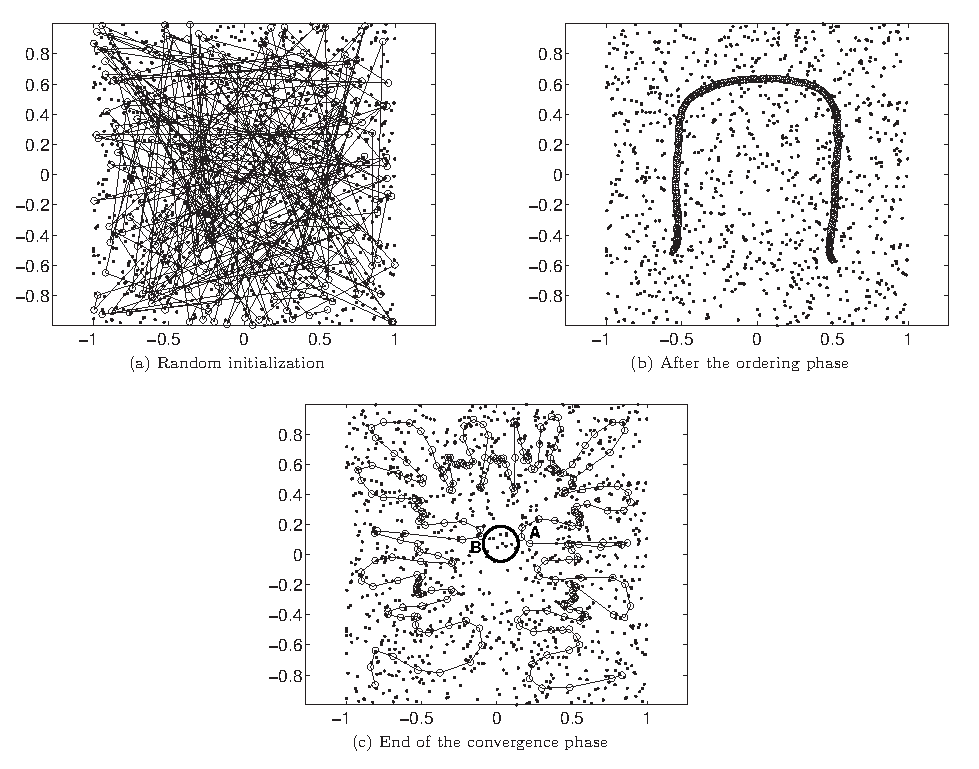
\includegraphics[width=1\textwidth]{SOM.eps}
%  \caption{}
\end{figure}
\newline Figure 1: An example of a one-dimensinal SOM with two-dimensional input data. In (c), the circle marks one area where the SOM mapping violates the topology of the input space.

\noindent \textbf{Computer exercises (one should select two or three to exercise)\\
9.2 (Hykin’s book, pp.480, 9.9) In this experiment we use computer simulations to investigate the SOM
algorithm applied to a one-dimensional lattice with a two-dimensional input. The lattice consists of 65
neurons. The inputs consist of random points uniformly distributed inside the triangular area shown in
Fig. Compute the map produced by the SOM algorithm after 20,100, 1000, 10000, and 25000
iterations respectively.}

\begin{figure}[!h]
  \centering
  \includegraphics[width=0.5\textwidth]{99.eps}
%  \caption{}\label{}
\end{figure}

~

\noindent First let's look at the generation of data and After normalization
\begin{figure}[!h]
  \centering
  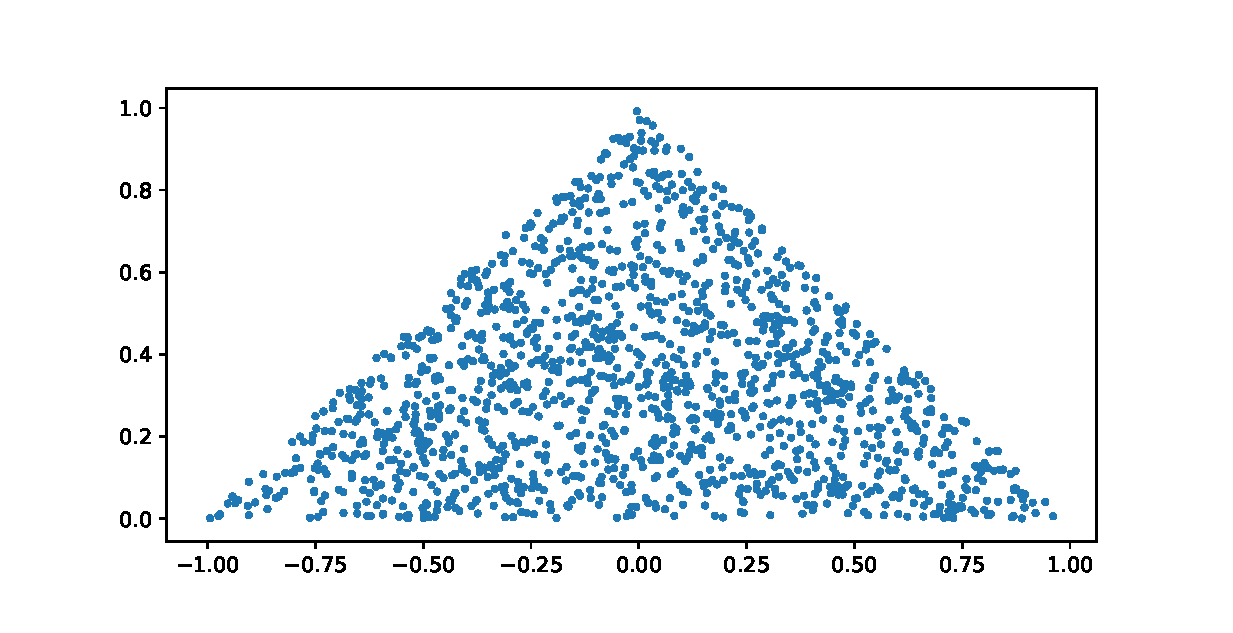
\includegraphics[width=0.6\textwidth]{data.eps}
%  \caption{}\label{}
\end{figure}

\noindent After normalization
\begin{figure}[!h]
  \centering
  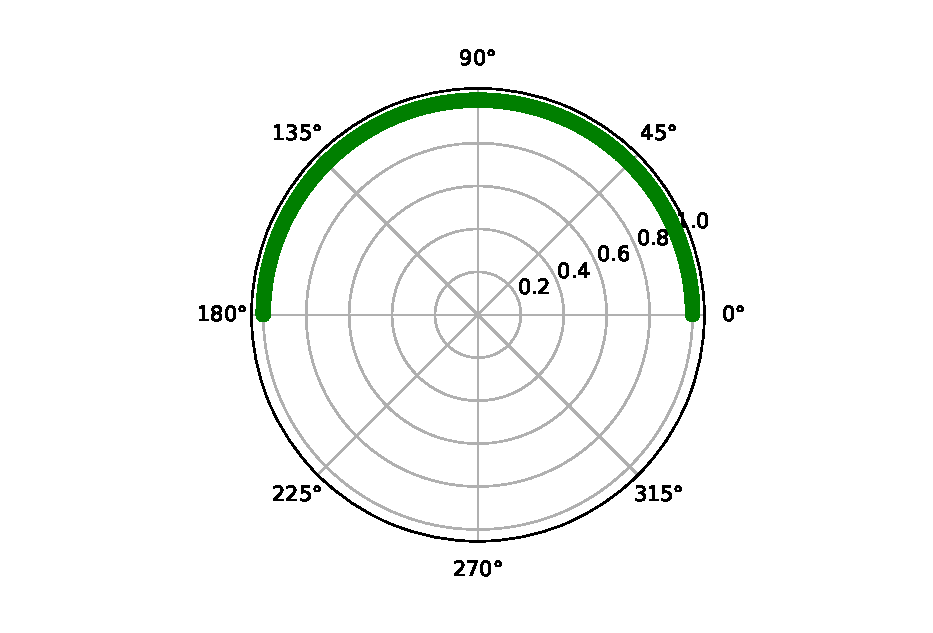
\includegraphics[width=0.6\textwidth]{polar.eps}
%  \caption{}\label{}
\end{figure}

\newpage
After initializing the weight vector and iteration 200,~1000,~10000,~25000,~30000.
\begin{figure}[!h]
\begin{minipage}
{0.5\linewidth}
\centering
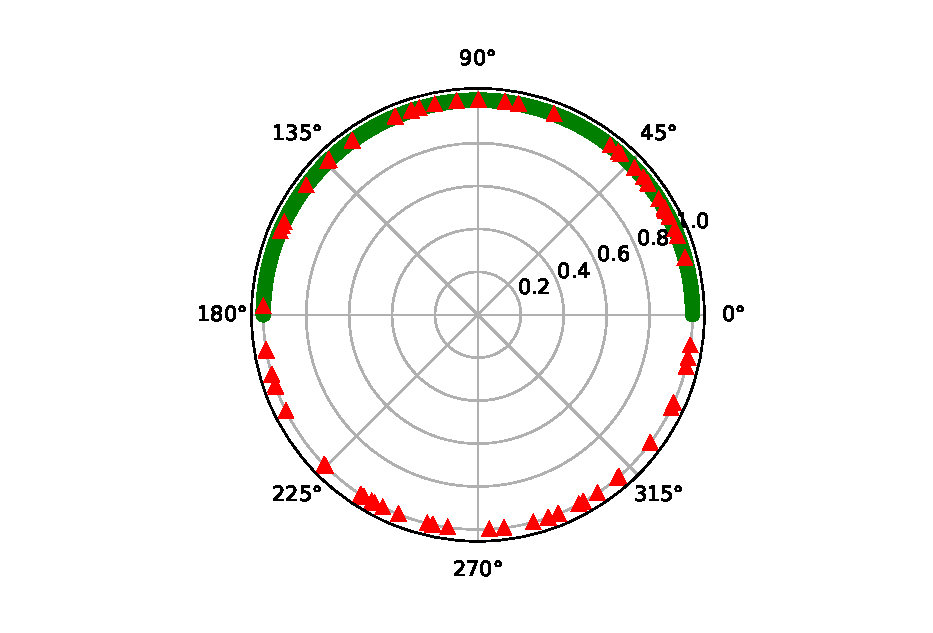
\includegraphics[width=3.5in]{initialization.eps}
\end{minipage}
%
\begin{minipage}
{0.5\linewidth}
\centering
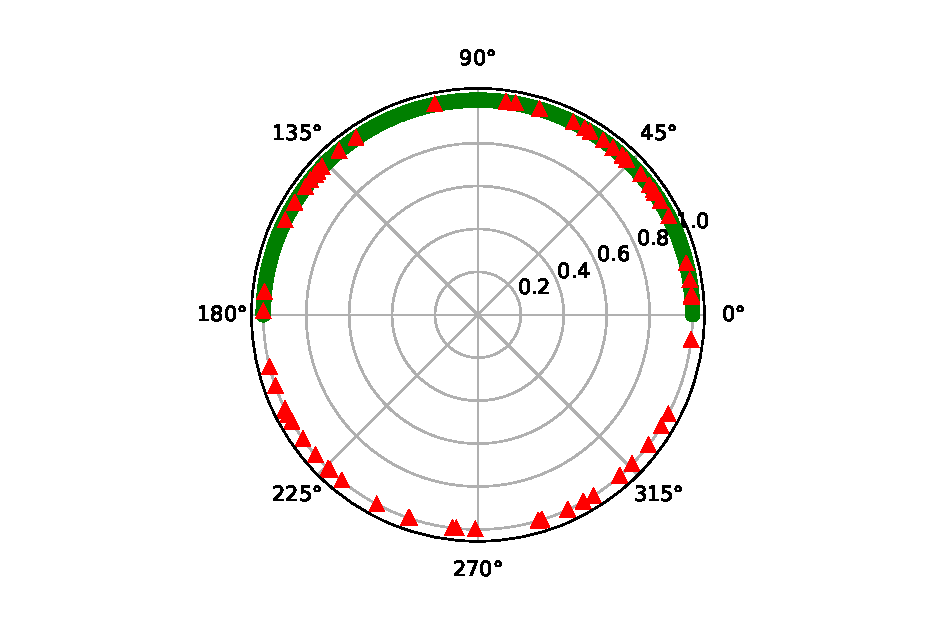
\includegraphics[width=3.5in]{20.eps}
\end{minipage}
\end{figure}

\begin{figure}[!h]
\begin{minipage}
{0.5\linewidth}
\centering
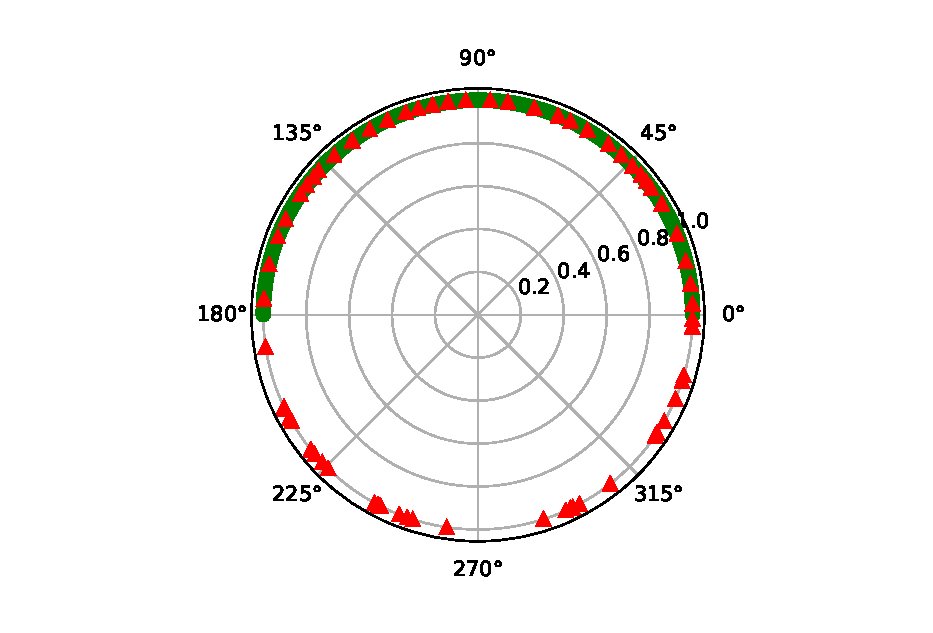
\includegraphics[width=3.5in]{1000.eps}
\end{minipage}
%
\begin{minipage}
{0.5\linewidth}
\centering
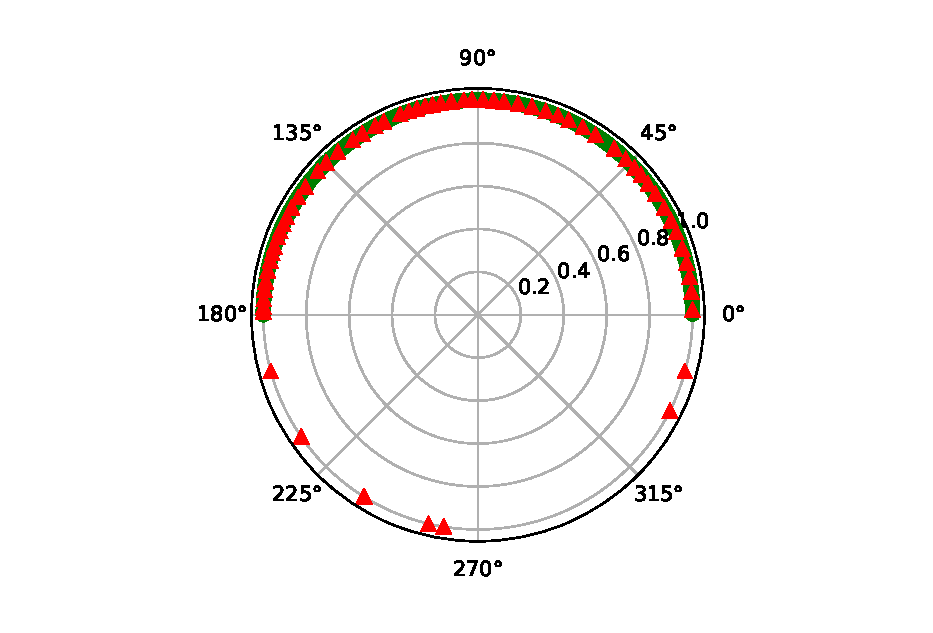
\includegraphics[width=3.5in]{30000.eps}
\end{minipage}
\end{figure}

\begin{figure}[!h]
\begin{minipage}
{0.5\linewidth}
\centering
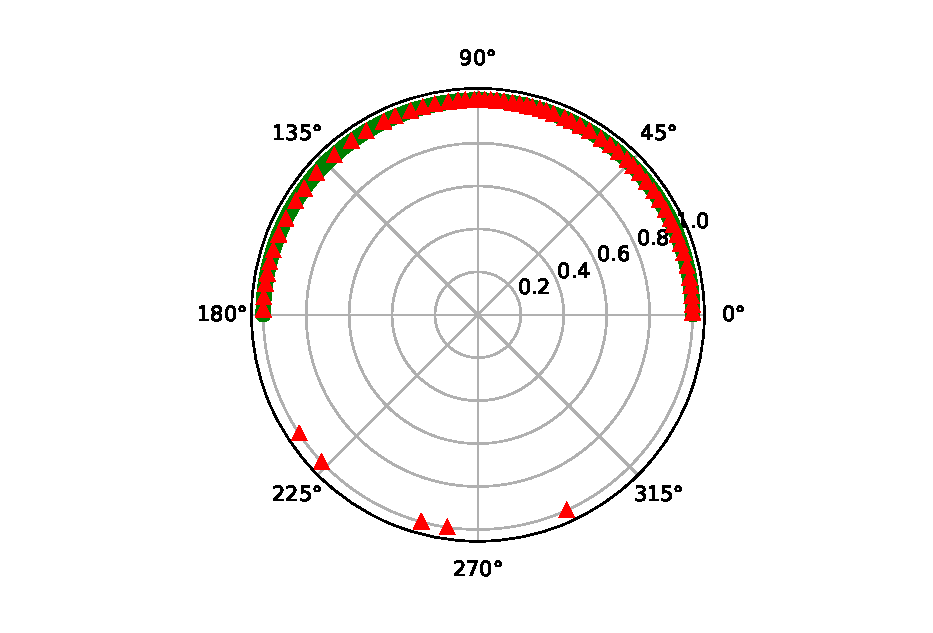
\includegraphics[width=3.5in]{25000.eps}
\end{minipage}
%
\begin{minipage}
{0.5\linewidth}
\centering
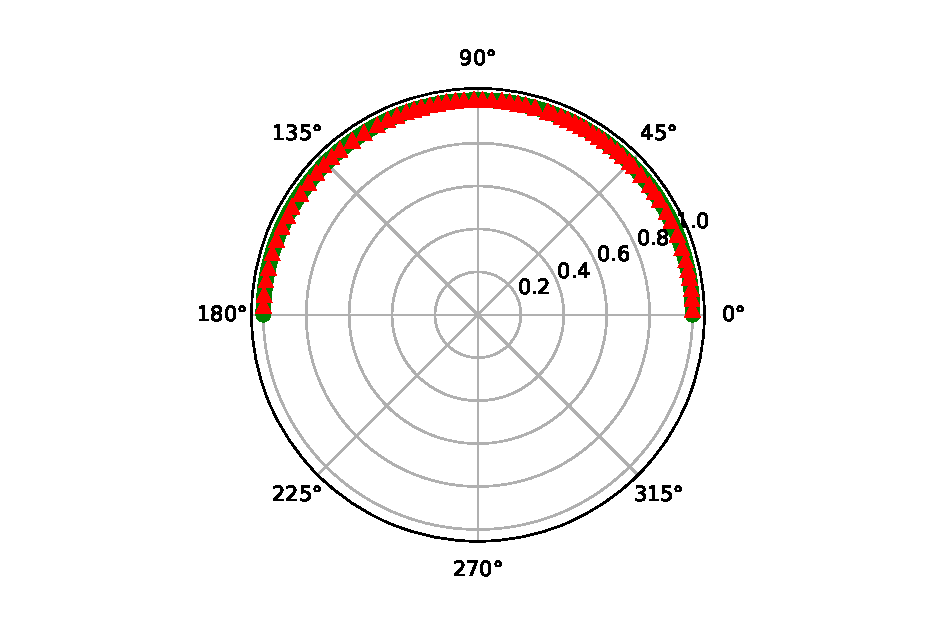
\includegraphics[width=3.5in]{40000.eps}
\end{minipage}
\end{figure}

This is the case of 65 neurons that produce a one-dimensional map.It can be seen that as the number of iterations increases, the algorithm converges slowly, and the weight vector distribution is close to the sample data distribution.
In fact, random initialization during the experiment may produce individual isolated points.
If the initialization in the sample will solve this problem.

Next, the mapping result of the two-dimensional mapping $20\times 20$ is shown.
\begin{figure}[!h]
  \centering
  \includegraphics[width=0.5\textwidth]{1.png}
\end{figure}

\begin{figure}[!h]
  \centering
  \includegraphics[width=0.5\textwidth]{3.png}
\end{figure}

The neurons with the same dimension as the sample can be seen that the distribution of the weight vector at the final convergence of the algorithm is close to the distribution of the sample data.

See the appendix for the procedure code.


\newpage
\noindent \textbf{9.3 (Dataset comes from Duda’s book, pp.681) Here is a dataset. Use SOM for the clustering of the data
in the dataset. Discuss the effect of structure of the SOM, and number of neurons in the SOM, and
visualize the learning process of the SOM by related matlab functions.}

\indent \indent \begin{tabular}{|c||c|c|c|}
  \hline
  % after \\: \hline or \cline{col1-col2} \cline{col3-col4} ...
  sample & $x_1$ & $x_2$ & $x_3$ \\
  \hline
  1 & -7.82 & -4.58 & -3.97 \\
  \hline
  2 & -6.68 & 3.16 & 2.71 \\
  \hline
  3 & 4.36 & -2.19 & 2.09 \\
  \hline
  4 & 6.72 & 0.88 & 2.80 \\
  \hline
  5 & -8.64 & 3.06 & 3.50 \\
  \hline
  6 & -6.87 & 0.57 & -5.45 \\
  \hline
  7 & 4.47 & -2.62 & 5.76 \\
  \hline
  8 & 6.73 & -2.01 & 4.18 \\
  \hline
  9 & -7.71 & 2.34 & -6.33 \\
  \hline
  10 & -6.91 & -0.49 & -5.68 \\
  \hline
\end{tabular}\indent
\begin{tabular}{|c||c|c|c|}
  \hline
  % after \\: \hline or \cline{col1-col2} \cline{col3-col4} ...
  sample & $x_1$ & $x_2$ & $x_3$ \\
  \hline
  11 & 6.18 & 2.81 & 5.82 \\
  \hline
  12 & 6.72 & -0.93 & -4.04 \\
  \hline
  13 & -6.25 & -0.26 & 0.56 \\
  \hline
  14 & -6.94 & -1.22 & 1.13 \\
  \hline
  15 & 8.09 & 0.20 & 2.25 \\
  \hline
  16 & 6.81 & 0.17 & -4.15 \\
  \hline
  17 & -5.19 & 4.24 & 4.04 \\
  \hline
  18 & -6.38 & -1.74 & 1.43 \\
  \hline
  19 & 4.08 & 1.30 & 5.33 \\
  \hline
  20 & 6.27 & 0.93 & -2.78 \\
  \hline
\end{tabular}
~\\

First data visualization.
\begin{figure}[!h]
\begin{minipage}
{0.5\linewidth}
\centering
\includegraphics[width=3in]{data1.eps}
\end{minipage}
%
\begin{minipage}
{0.5\linewidth}
\centering
\includegraphics[width=3in]{2_1.eps}
\end{minipage}
\end{figure}

Because the data is very small, we can only give fewer neurons.
First data visualization
and set of $2\times1$ neurons is found to converge quickly as shown above.

\newpage
Then set up three mode classes.Due to the random initialization of the weight variable, the final convergence causes three modes of the two modes. Because the data is scarce, the performance of the two types is difficult to distinguish.
\begin{figure}[!h]
\begin{minipage}
{0.5\linewidth}
\centering
\includegraphics[width=3in]{3_1_1000.eps}
\end{minipage}
%
\begin{minipage}
{0.5\linewidth}
\centering
\includegraphics[width=3in]{3_1_10000.eps}
\end{minipage}
\end{figure}


Finally, after exploring, we set 8 pattern classes relatively well, and it is easy to complete clustering after a few iterations.
\begin{figure}[!h]
\begin{minipage}
{0.5\linewidth}
\centering
\includegraphics[width=3in]{4_2_1.eps}
\end{minipage}
%
\begin{minipage}
{0.5\linewidth}
\centering
\includegraphics[width=3in]{4_2_10.eps}
\end{minipage}
\end{figure}
\begin{figure}[!h]
\begin{minipage}
{0.5\linewidth}
\centering
\includegraphics[width=3in]{4_2_100.eps}
\end{minipage}
%
\begin{minipage}
{0.5\linewidth}
\centering
\includegraphics[width=3in]{4_2_1000.eps}
\end{minipage}
\end{figure}

See the appendix for the procedure code.

\newpage
\noindent \textbf{9.4 Generate randomly 100 samples (cities) in the square of $[0,1]^2$. Now construct a circular SOM and a
linear SOM respectively with 130 neurons initialized randomly in the square of the $[0,1]^2$, learn the
SOM with the 100 cities, and visualize the learning process of the SOM to see what the route defined by
the converged neurons like. Is it a roughly approximate solution of the TSP (traveling salesman problem)
and/or SP (shortest path problem) defined by the cities?}








